\documentclass[final]{beamer}
\usepackage[size=custom,width=91.44,height=60.96,scale=1.0]{beamerposter} % if you change this, also change the 
\usepackage{uscPosterTheme} % Assuming this is adjusted to not redefine colors but to include layout and font settings
\usepackage{uscColor} % Load USC color theme

%==================
%  Bibliography
%==================
\usepackage[backend=biber, style=numeric-comp, citestyle=numeric-comp]{biblatex} % Currently set up for Biblatex
\addbibresource{references.bib}

\AtBeginBibliography{\scriptsize} % Set the size of the script


\title{Your Poster Title}
\author{Your Name}
\date{\today}

% Your document content

\title{Research Poster Title}
\author{Author Name}
\institute{University of Southern California}
\date{\today}

\begin{document}

\begin{frame}[t]

\begin{center}

    \Huge \garamondfont\textbf{\inserttitle}\\[-8pt]
    
    \huge \insertauthor\\[-7pt]
    
    \normalsize \insertdate
    
\end{center}

\begin{columns}[t]

% First column
\begin{column}{.30\textwidth}
\begin{block}{Introduction}
    Lorem ipsum dolor sit amet, consectetur adipiscing elit. Duis dui odio, volutpat vitae sapien sed, elementum iaculis sem \cite{lee_cross-sectional_2017}. Nulla ac tellus purus. Nam aliquam sem purus, sed consequat felis ultricies auctor. Fusce sodales, sapien eget mollis sodales, ex urna sollicitudin tellus, ac molestie ligula ligula at ante. Duis vestibulum lorem odio, ut tincidunt nulla ultrices eget. Aliquam laoreet imperdiet scelerisque. Etiam sapien turpis, pulvinar vel libero quis, tincidunt laoreet ante \cite{jackson_estimation_2015}. Vivamus tortor ante, hendrerit eget diam quis, ultricies pretium velit. Nullam vestibulum velit id lacus aliquet vulputate. Maecenas id accumsan lectus, eu pellentesque lacus. Suspendisse quis mi sit amet arcu faucibus tincidunt ut vel urna. Nunc finibus magna sit amet hendrerit maximus. Etiam ut mi in est facilisis laoreet. Phasellus vitae mi lacus. In mattis at ex non vehicula. In libero magna, tempus non lacus ut, sollicitudin viverra neque.

    \begin{equation} \label{fig:sample_equation}
        f(x_{0},y_{0}) = 
        \begin{dcases}
            \frac{1}{2\pi r\sqrt{x_{0}^{2}+y_{0}^{2}}}, & \text{if } \sqrt{x_{0}^2 + y_{0}^2} \leq r\\
            0, & \text{otherwise}
        \end{dcases}
    \end{equation}

    Sed sed sapien dolor. Donec suscipit lectus est, dictum facilisis velit facilisis ac. Duis placerat, ex eget malesuada accumsan, erat nibh placerat sapien, luctus vehicula leo libero pellentesque tortor. In rutrum cursus arcu. Sed sed imperdiet dui. Curabitur auctor elit lorem, eu porttitor risus sollicitudin vitae. Donec viverra lacus id urna mattis faucibus. Vivamus egestas lectus lorem, a finibus arcu posuere a. Vestibulum ante ipsum primis in faucibus orci luctus et ultrices posuere cubilia curae; Proin fringilla pellentesque justo, semper consectetur nisl facilisis id \cite{stones_access_2018}. Aliquam erat volutpat. Nam porta odio et velit eleifend, at tempus quam faucibus. Etiam id finibus neque, vel lacinia ex. Curabitur dictum ligula vitae tellus sodales rutrum.

\end{block}

\begin{block}{Background}
  Duis bibendum lorem non nulla sagittis, at maximus lectus aliquet. Ut dictum varius viverra. Aenean sed semper turpis, eu faucibus urna. Suspendisse potenti. Etiam nec felis in orci euismod laoreet id ut tellus. Maecenas risus purus, fermentum sit amet convallis et, dignissim eu est. Praesent id gravida mauris. 
\end{block}
\end{column}

% Second column
\begin{column}{.30\textwidth}
\begin{block}{Methodology}
  Describe research methods here.

  \vspace*{0.75in}

      \begin{figure}
        \centering
        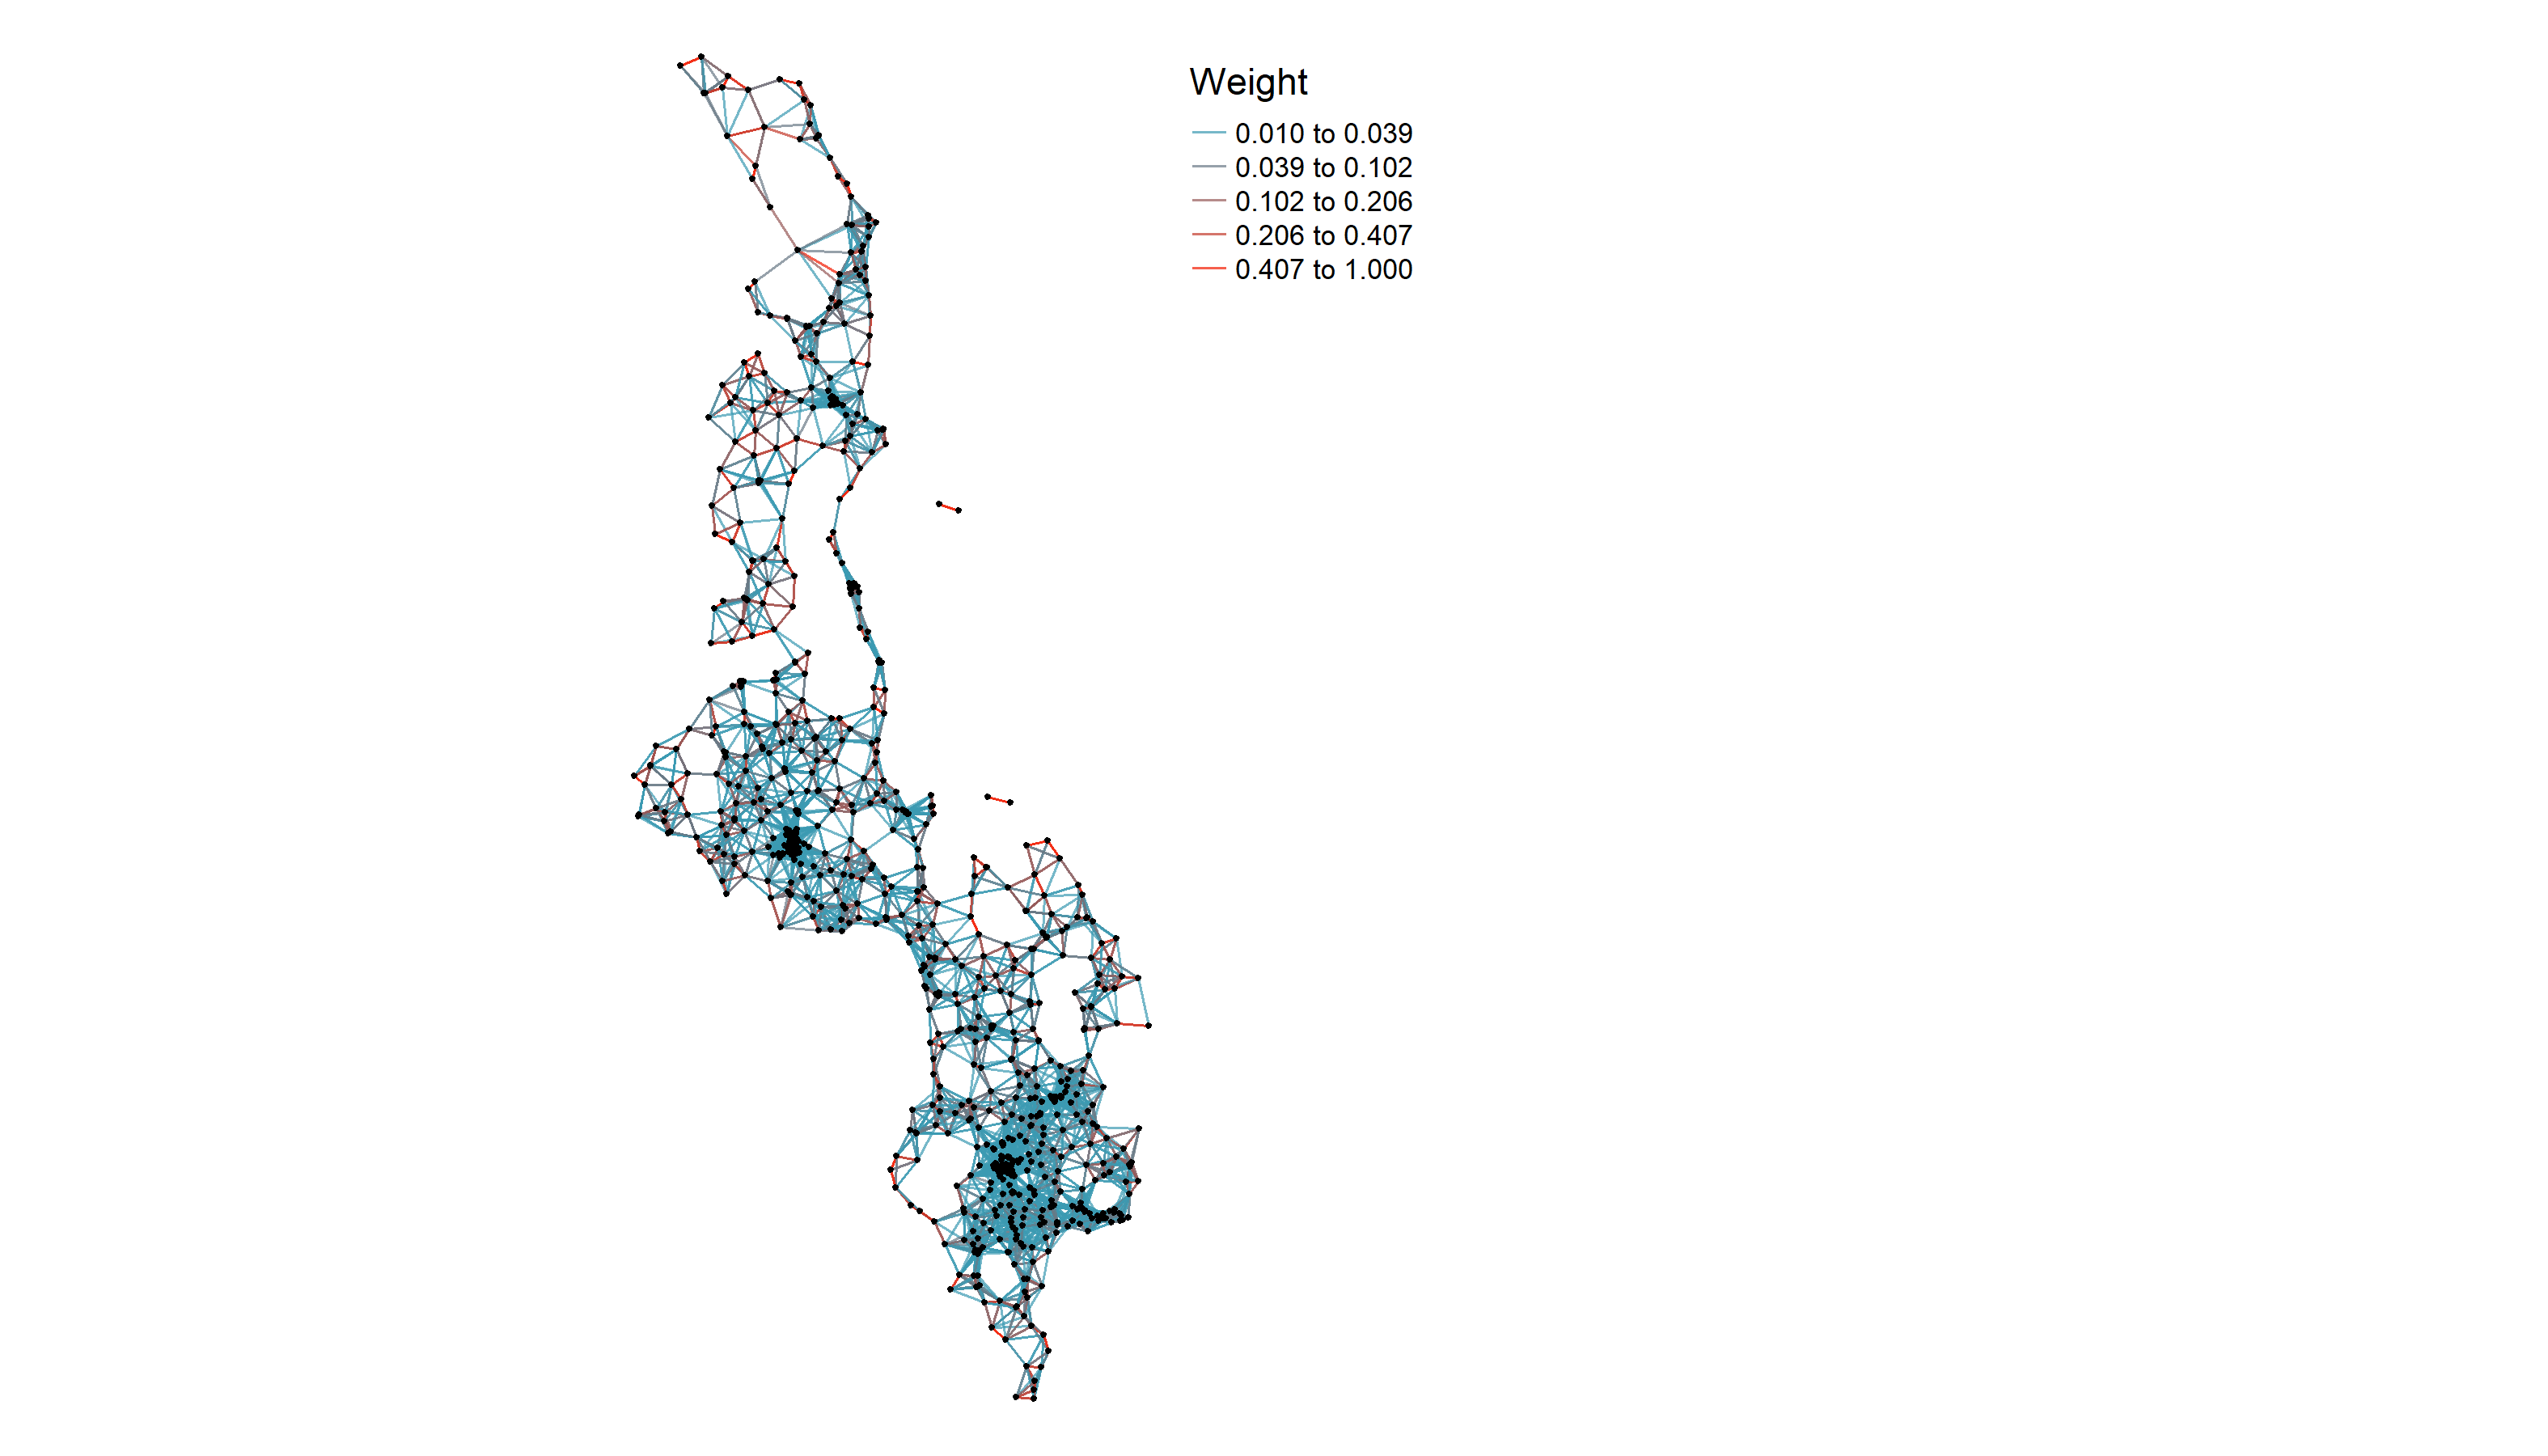
\includegraphics[width=\textwidth]{images/figures/map_network_gauss.png}
        \caption{Example of an included figure}
        \label{fig:example_fig}
    \end{figure}
    
\end{block}



\begin{block}{Results}
  Lorem ipsum dolor sit amet, consectetur adipiscing elit. Morbi consectetur vitae felis sit amet eleifend. Ut tristique interdum urna, at sodales dolor lobortis sed. Nullam convallis, magna eget placerat congue, arcu ligula gravida ligula, vitae faucibus orci turpis nec nisi. Maecenas auctor elementum sodales. Nulla ultrices lorem at lectus sodales ultricies. Aliquam congue leo at mi congue aliquam. Cras ut posuere lectus. Phasellus fringilla, dui non elementum viverra, lorem purus efficitur arcu, gravida varius felis ligula ac urna. Suspendisse a auctor mi, a sollicitudin nulla. Ut tortor dui, accumsan sit amet elementum ultrices, gravida at erat. Nunc tincidunt fermentum ligula.
\end{block}
\end{column}

% Third column
\begin{column}{.30\textwidth}

\begin{exampleblock}{This is an example}
     Lorem ipsum dolor sit amet, consectetur adipiscing elit. Duis dui odio, volutpat vitae sapien sed, elementum iaculis sem. Nulla ac tellus purus. Nam aliquam sem purus, sed consequat felis ultricies auctor. 
     
    {\small
     \begin{table}[!htbp] \centering 
     \caption{Results compared} \label{tab:fittedModels} 
        \begin{tabular}{@{\extracolsep{5pt}}lcccc} 
            \\[-1.8ex]\hline 
            \hline \\[-1.8ex] 
            & \multicolumn{4}{c}{\textit{Dependent variable:}} \\ 
            \cline{2-5} 
            \\[-1.8ex] & \multicolumn{2}{c}{4+ ANC visits} & \multicolumn{2}{c}{Current MFP Use}  \\ 
            \\[-1.8ex] & (PWM) & (BM)\dag & (PWM) & (BM)\dag \\ 
            \hline \\[-1.8ex] 
            SRI Score & 0.150$^{***}$ & 0.181$^{***}$ & 0.100$^{***}$ & 0.098$^{*}$ \\
            Travel time minutes (log transformed) & $-$0.268$^{***}$ & $-$0.300$^{***}$ & $-$0.015 & $-$0.034 \\ 
            \hline \\[-1.8ex] 
            Akaike Inf. Crit. & 4,113.977 & 4,115.690 & 8,224.051 & 8,227.574 \\ 
            \hline 
            \hline \\[-1.8ex]
            \multicolumn{5}{l}{$^{*}$p$<$0.1; $^{**}$p$<$0.05; $^{***}$p$<$0.01} \\ 
            \multicolumn{5}{l}{\footnotesize \dag PWM: This is an example note.}\\
        \end{tabular} 
    \end{table} 
    }

    Fusce sodales, sapien eget mollis sodales, ex urna sollicitudin tellus, ac molestie ligula ligula at ante.
    
\end{exampleblock}

% Discussion block

\begin{block}{Conclusion}
  Donec ac urna non tellus consequat facilisis. Duis egestas vehicula lectus, ut egestas metus tempor a. Aenean eu neque odio. Curabitur fermentum, arcu ut venenatis porttitor, mauris odio fringilla dui, in tincidunt nisi enim quis sem. Vivamus finibus pulvinar libero.
\end{block}

% References
\begin{block}{References}

    {
    \printbibliography
    }
     
\end{block}

\end{column}

\end{columns}

\end{frame}

\end{document}
